% Compile with: latexmk -pdf example.tex
% The content is original demonstration material, not copied book text.
\documentclass{hubbardbook}
\usepackage{tikz}
\usetikzlibrary{arrows.meta}
\newcommand{\R}{\mathbb{R}}
\newcommand{\norm}[1]{\lVert #1\rVert}
\newcommand{\inner}[2]{\langle #1,#2\rangle}
\hypersetup{pdftitle={A mathematics book: layout specimen},
  pdfauthor={Hubbard-style LaTeX template}}

\begin{document}
\mainmatter
\chapter{Vectors and linear maps}
\chapterepigraph{A useful definition should help us compute,\newline
but it should also help us see.}{A guiding principle for this example}

\introsection
\sidenote{This example shows the fixed left sidebar and the book's
section-based numbering. It uses Computer Modern for text and mathematics.
The sample text and drawings are original.}
Linear algebra studies operations that preserve addition and scalar
multiplication. These operations occur whenever several quantities are
combined without interaction terms: adding displacements, changing
coordinates, or superposing solutions of a homogeneous equation.

The point of introducing an abstract definition is to recognize the same
structure in different settings. A column of numbers, a polynomial, and a
continuous function can all be vectors. Their concrete descriptions differ,
but many of the arguments we make about them are identical.

We move between coordinates and geometry. The main column develops the
argument; the margin supplies interpretations and reminders.

\section{Vectors and length}
\label{sec:vectors}
A point describes a location; a vector describes a displacement. After
choosing an origin, we may represent both by the same list of coordinates,
but it is useful to remember their different roles. We can add two
displacements without making any further choice.

\begin{definition}[Euclidean inner product]\label{def:inner}
For \(u,v\in\R^n\), their \emph{inner product} is
\begin{equation}\label{eq:inner}
  \inner{u}{v}=\sum_{j=1}^{n}u_jv_j.
\end{equation}
The associated length is \(\norm{v}=\sqrt{\inner{v}{v}}\).
\end{definition}

\sidenote{For a nonzero vector, length and direction carry different
information. Dividing by the length produces a unit vector with the same
direction.}
The inner product is linear in each variable and symmetric in its two
arguments. It is also positive: \(\inner{v}{v}\geq0\), with equality
precisely when every coordinate of \(v\) vanishes. These observations
follow directly from the coordinate formula.

\begin{example}[A unit vector]
The vector \(v=(3,4)\) has length \(5\). Therefore
\(\frac15v=(\frac35,\frac45)\) has length \(1\).
\end{example}

\clearpage
\subsection{A geometric interpretation}
\begin{marginfigure}
\centering
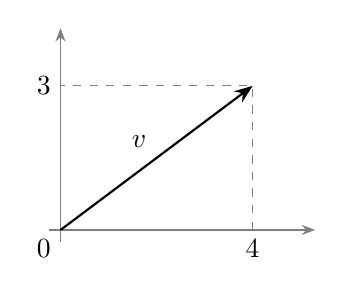
\begin{tikzpicture}[scale=0.61,>=Stealth]
  \draw[->,gray] (-.25,0)--(5.3,0);
  \draw[->,gray] (0,-.25)--(0,4.2);
  \draw[dashed,gray] (4,0)--(4,3)--(0,3);
  \draw[->,thick] (0,0)--(4,3) node[midway,above left]{\(v\)};
  \node[below] at (4,0){\(4\)};
  \node[left] at (0,3){\(3\)};
  \node[below left] at (0,0){\(0\)};
\end{tikzpicture}
\caption{The vector \(v=(4,3)\) and its coordinate displacements.}
\label{fig:vector}
\end{marginfigure}
In the plane, the coordinate formula for length is the Pythagorean
theorem. Figure~\ref{fig:vector} separates a displacement into horizontal
and vertical parts. The same formula in higher dimensions adds the squares
of all the coordinate displacements.

Angles can also be recovered from the inner product. For nonzero vectors
\(u\) and \(v\), the cosine of the angle between them is
\begin{equation}\label{eq:angle}
  \cos\theta=\frac{\inner{u}{v}}{\norm{u}\,\norm{v}}.
\end{equation}
The following inequality ensures that the quotient lies in \([-1,1]\).
It will also give us the triangle inequality, which expresses the fact
that traveling directly is no longer than traveling in two stages.

\begin{theorem}[Cauchy--Schwarz inequality]\label{thm:cs}
For all \(u,v\in\R^n\),
\begin{equation}\label{eq:cs}
  |\inner{u}{v}|\leq\norm{u}\,\norm{v}.
\end{equation}
\end{theorem}
\begin{proof}
The result is immediate if \(v=0\). Otherwise, for every real \(t\),
\begin{align*}
  0&\leq\norm{u-tv}^2\\
   &=\norm{u}^2-2t\inner{u}{v}+t^2\norm{v}^2.
\end{align*}
Set \(t=\inner{u}{v}/\norm{v}^2\). Substitution gives
\(0\leq\norm{u}^2-\inner{u}{v}^2/\norm{v}^2\), which is the desired
inequality after multiplication and taking square roots.
\end{proof}

\sidenote{Equality in Cauchy--Schwarz occurs when the vectors are linearly
dependent. In the proof, it occurs when the residual vector \(u-tv\)
can be made zero.}
\begin{corollary}[Triangle inequality]\label{cor:triangle}
For all \(u,v\in\R^n\),
\(\norm{u+v}\leq\norm{u}+\norm{v}\).
\end{corollary}
\begin{proof}
Expand the square of the left side and apply Theorem~\ref{thm:cs}:
\[
  \norm{u+v}^2
  \leq\norm{u}^2+2\norm{u}\,\norm{v}+\norm{v}^2
  =(\norm{u}+\norm{v})^2.
\]
Both sides are nonnegative, so we may take square roots.
\end{proof}

\begin{remark*}
A coordinate formula can suggest a geometric statement; a geometric
picture can suggest the right algebraic proof. Neither viewpoint needs
to replace the other.
\end{remark*}

\clearpage
\section{Linear maps}
\label{sec:linear}
\sidenote{The same definition applies to arbitrary real vector spaces.
Coordinates are convenient for calculation, but they are not part of the
underlying idea of linearity.}
The operations of addition and scalar multiplication determine what a
linear map must preserve. One compact identity expresses both requirements.

\begin{definition}[Linear map]\label{def:linear}
A map \(T\colon\R^n\to\R^m\) is \emph{linear} if
\begin{equation}\label{eq:linear}
  T(au+bv)=aT(u)+bT(v)
\end{equation}
for every \(u,v\in\R^n\) and every \(a,b\in\R\).
\end{definition}

\begin{example}[A shear]\label{ex:shear}
The map \(S(x,y)=(x+y,y)\) is linear. It leaves the horizontal axis
fixed and shifts every other horizontal line by an amount proportional
to its height. Its matrix in the standard basis is
\begin{equation}\label{eq:shear}
  A=\begin{pmatrix}1&1\\0&1\end{pmatrix},
  \qquad S\begin{pmatrix}x\\y\end{pmatrix}
  =A\begin{pmatrix}x\\y\end{pmatrix}.
\end{equation}
\end{example}

\begin{figure}[htbp]
\centering
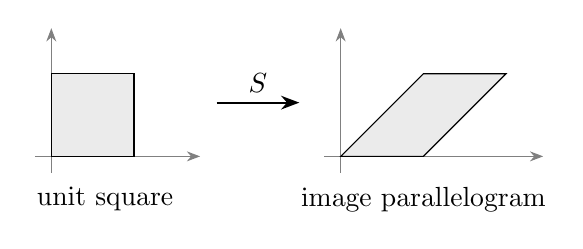
\begin{tikzpicture}[scale=1.05,>=Stealth]
  \begin{scope}
    \draw[->,gray] (-.2,0)--(1.8,0);
    \draw[->,gray] (0,-.2)--(0,1.55);
    \filldraw[fill=black!8] (0,0)--(1,0)--(1,1)--(0,1)--cycle;
    \node[below] at (.65,-.25){unit square};
  \end{scope}
  \draw[->,thick] (2,.65)--(3,.65) node[midway,above]{\(S\)};
  \begin{scope}[xshift=3.5cm]
    \draw[->,gray] (-.2,0)--(2.45,0);
    \draw[->,gray] (0,-.2)--(0,1.55);
    \filldraw[fill=black!8] (0,0)--(1,0)--(2,1)--(1,1)--cycle;
    \node[below] at (1,-.25){image parallelogram};
  \end{scope}
\end{tikzpicture}
\caption{A shear changes angles while preserving parallel lines and area.}
\label{fig:shear}
\end{figure}

\subsection{What happens to the origin?}
\sidenote{A translation \(x\mapsto x+c\), with \(c\neq0\), is not linear:
it moves the origin. It is an affine map. This distinction matters even
when the graph looks like a straight line.}
\begin{proposition}\label{prop:zero}
Every linear map sends the zero vector to the zero vector.
\end{proposition}
\begin{proof}
Since \(0=0+0\), linearity gives \(T(0)=T(0)+T(0)\).
Subtracting \(T(0)\) proves the claim.
\end{proof}

\begin{textblock}{A useful test}
Before checking the full definition, evaluate the proposed map at zero.
If the result is nonzero, the map cannot be linear.
\end{textblock}

\clearpage
\subsection{Matrices encode the images of a basis}
Let \(e_1,\ldots,e_n\) be the standard basis. Every vector has the
expansion \(v=\sum_jv_je_j\). If \(T\) is linear, we therefore have
\begin{equation}\label{eq:basis}
  T(v)=\sum_{j=1}^{n}v_jT(e_j).
\end{equation}
The vectors \(T(e_j)\) completely determine the map. Arrange them as the
columns of a matrix \(A\); equation~\ref{eq:basis} then says \(T(v)=Av\).

\autonote{This is an automatically placed note. It can move downward to
avoid another automatic note. It is useful when exact vertical alignment
is less important than keeping a sequence of notes apart.}
\begin{boxedtheorem}[Basis criterion]\label{thm:basis}
Two linear maps \(T,U\colon\R^n\to\R^m\) are equal if and only if
\(T(e_j)=U(e_j)\) for every standard basis vector \(e_j\).
\end{boxedtheorem}
\begin{proof}
One direction is immediate. For the other, expand an arbitrary vector
in the standard basis and use linearity:
\[
  T(v)=\sum_jv_jT(e_j)=\sum_jv_jU(e_j)=U(v).
\]
Thus the two maps agree at every vector.
\end{proof}

\begin{textbox}{Reading a matrix by columns}
The \(j\)th column answers a concrete question: where does the map send
the \(j\)th basis vector? This interpretation is often easier to remember
than a formula involving two indices.
\end{textbox}

\begin{shadedbox}{Common pitfall}
Preserving lengths is a much stronger requirement than being linear.
The shear in Example~\ref{ex:shear} is linear, but it sends \((0,1)\)
to \((1,1)\), changing the length from \(1\) to \(\sqrt2\).
\end{shadedbox}

\begin{exercises}
\begin{exercise}\label{exercise:zero}
Show that every linear map satisfies \(T(-v)=-T(v)\).
\end{exercise}
\begin{exercise}
Find the matrix of \(T(x,y)=(2x-y,x+3y)\). What are the images of
the two standard basis vectors?
\end{exercise}
\begin{exercise}[Composition]
Prove that the composition of two linear maps is linear. If their
matrices are \(A\) and \(B\), in that order, what is the matrix of
the composition?
\end{exercise}
\begin{exercise}
Give a map \(f\colon\R\to\R\) that fixes zero but is not linear.
\end{exercise}
\end{exercises}

\chapter{Orthogonal decomposition}
\chapterepigraph{Choose the component that explains the direction,\newline
then study what remains.}{A second viewpoint}

\introsection
Many calculations become simpler after splitting a vector into two
perpendicular pieces. One piece lies in a chosen direction; the other
records the residual. This is the basic geometry behind projection and
least-squares approximation.

\section{Projection onto a line}
Fix a nonzero vector \(u\). We seek a scalar \(a\) for which
\(v-au\) is perpendicular to \(u\). The condition
\(\inner{v-au}{u}=0\) gives a unique answer.

\sidenote{The denominator is \(\norm{u}^2\), so the expression is defined
only when \(u\neq0\). Multiplying \(u\) by a nonzero scalar does not
change the projection map.}
\begin{definition}[Orthogonal projection]\label{def:projection}
The projection of \(v\) onto the line spanned by \(u\neq0\) is
\begin{equation}\label{eq:projection}
  P_u(v)=\frac{\inner{v}{u}}{\inner{u}{u}}\,u.
\end{equation}
\end{definition}

The map \(P_u\) is linear. Moreover, \(P_u(v)\) lies on the chosen
line and \(v-P_u(v)\) is perpendicular to it. These properties
characterize the decomposition uniquely.

\begin{theorem}[Best approximation]\label{thm:best}
Among all vectors \(w\) on the line spanned by \(u\), the vector
\(P_u(v)\) uniquely minimizes \(\norm{v-w}\).
\end{theorem}
\begin{proof}
Write \(v-w=(v-P_u(v))+(P_u(v)-w)\). The two summands are
perpendicular, so
\[
  \norm{v-w}^2=\norm{v-P_u(v)}^2+\norm{P_u(v)-w}^2.
\]
The final term is nonnegative and vanishes exactly when \(w=P_u(v)\).
\end{proof}

\begin{remark*}
This is a geometric optimization argument: perpendicularity converts
the quantity being minimized into a fixed term plus a nonnegative term.
\end{remark*}

\clearpage
\subsection{Seeing the residual}
The following drawing occupies both columns. A wide figure is useful
when the relation between several objects would be cramped in the main
column. Leave the corresponding margin area free of notes.

\begin{fullwidth}
\begin{center}
\begin{tikzpicture}[scale=1.0,>=Stealth]
  \draw[gray,->] (-.6,0)--(10.5,0) node[right]{line spanned by \(u\)};
  \draw[->,very thick] (0,0)--(5.8,2.8) node[midway,above left]{\(v\)};
  \draw[->,thick] (0,0)--(5.8,0) node[midway,below]{\(P_u(v)\)};
  \draw[->,thick] (5.8,0)--(5.8,2.8)
    node[midway,right]{\(v-P_u(v)\)};
  \draw (5.5,0)--(5.5,.3)--(5.8,.3);
  \fill (0,0) circle (1.4pt) node[below left]{\(0\)};
\end{tikzpicture}
\end{center}
\captionsetup{hypcap=false}
\captionof{figure}{An orthogonal decomposition into a component on a line
and a residual perpendicular to it. The caption and diagram use the full width.}
\label{fig:projection}
\end{fullwidth}

\medskip
Applying the projection twice has the same effect as applying it once:
\begin{equation}\label{eq:idempotent}
  P_u^2=P_u.
\end{equation}
A map with this property is called \emph{idempotent}. Once a vector has
landed on the chosen line, a further projection leaves it unchanged.

\subsection{A numerical example}
\numberedsidenote{A margin note can also carry a number. The reference
mainly uses unnumbered notes. Ordinary footnotes remain available.}
Let \(u=(1,1)\) and \(v=(2,0)\). Then \(P_u(v)=(1,1)\), and the
residual is \((1,-1)\). Their inner product is zero, as expected.
The squared length of \(v\) is \(4\); the squared lengths of its
two perpendicular components are \(2\) and \(2\).

\begin{boxeddefinition}[Idempotent map]
A linear map \(P\colon V\to V\) is \emph{idempotent} if \(P^2=P\).
\end{boxeddefinition}

\begin{exercises}
\begin{exercise}
Verify directly from equation~\ref{eq:projection} that \(P_u^2=P_u\).
\end{exercise}
\begin{exercise}
Find the matrix of the orthogonal projection onto the line spanned by
\((1,2)\). Check that the matrix is symmetric and idempotent.
\end{exercise}
\end{exercises}
\end{document}
